\documentclass{beamer}
\usepackage[utf8]{inputenc}
\usepackage{graphicx}
\usepackage{listings}
\usepackage{mathtools}

% Chart plotting
\usepackage{tikz}
\usepackage{pgfplots}
\usetikzlibrary{matrix,snakes,patterns}
\usetikzlibrary{decorations.pathmorphing}
\usetikzlibrary{decorations.markings}
\usetikzlibrary{plotmarks}
\tikzstyle{inChart}=[anchor=north east]
\tikzstyle{grid}=[loosely dotted] % [ultra thin] % % [dotted]
\newcommand{\subt}[3] { 
  \draw[grid] (#1,#1) -- (#1,#2) node[inChart] {#3} -- (#2,#2);
  \fill[color=black] (#1,#2) circle (2pt)
 }
\newcommand{\mrk}[2]{\node[inChart] at (#1,#1) {#2}}

% Haskell (and other) source code listing
\lstloadlanguages{Haskell}
\lstnewenvironment{code}
    {\lstset{}%
      \csname lst@SetFirstLabel\endcsname}
    {\csname lst@SaveFirstLabel\endcsname}
    \lstset{
      basicstyle=\small\ttfamily,
      flexiblecolumns=false,
      basewidth={0.5em,0.45em},
      literate={+}{{$+$}}1 {/}{{$/$}}1 {*}{{$*$}}1 {=}{{$=$}}1
               {>}{{$>$}}1 {<}{{$<$}}1 {\\}{{$\lambda$}}1
               {\\\\}{{\char`\\\char`\\}}1
               {->}{{$\rightarrow$}}2 {>=}{{$\geq$}}2 {<-}{{$\leftarrow$}}2
               {<=}{{$\leq$}}2 {=>}{{$\Rightarrow$}}2 
               {\ .}{{$\circ$}}2 {\ .\ }{{$\circ$}}2
               {>>}{{>>}}2 {>>=}{{>>=}}2
               {|}{{$\mid$}}1               
    }

\usetheme{Warsaw}

\title{Implementing incremental and parallel parsing}
\author{Tobias Olausson}
\institute{University of Gothenburg}
\date{May 22, 2014}

\begin{document}

\begin{frame}
\titlepage
\end{frame}

\begin{frame}{In this talk}
    \begin{itemize}
        \item Parsing using the CYK algorithm
        \item Implementing an incremental parser
        \item Writing dependently typed Haskell code
        \item ...and a lot of itemized lists
    \end{itemize}
\end{frame}

\section{Background}
\begin{frame}{Motivation}
    \begin{itemize}
        \item Parallelism everywhere \\
              $\rightarrow$ divide-and-conquer algorithms suitable
        \item Syntax highlighting sucks
        \item Parsing is usually linear-ish
    \end{itemize}
    We can do better!
\end{frame}

\subsection{Context-free grammars}
\begin{frame}{Context-free grammars}
    \begin{itemize}
        \item 4-tuple: $G = (V, \Sigma, P, S)$
        \begin{itemize}
            \item $V$ set of variables
            \item $\Sigma$ set of terminal symbols
            \item $P$ productions, recursive rules
            \item $S$ start symbol, entrypoint
        \end{itemize}
        \item Backus-Naur Form \\
              $A ::= a$ \\ 
              $A ::= BC$
    \end{itemize}
\end{frame}

\subsection{CYK algorithm}
\begin{frame}{CYK algorithm}
    \begin{itemize}
        \item Cocke, Younger and Kasami (60s)
        \item Grammar in Chomsky Normal Form \\
              $\rightarrow$ Only binary or unary rules
        \item Recognition matrix
        \item Not very efficient, $O(n^3)$
    \end{itemize}
\end{frame}

\begin{frame}{How does it work?}
  \begin{columns}[c]
  \begin{column}{.5\textwidth}

    \begin{align*}
    W_{i,i+1} &= \{ A | A ::= S_t[i] \in P \} \\
    W_{ij}    &= \sum_{k=i+1}^{j} W_{ik} \cdot W_{kj} \\
    x \cdot y &= \{ A | A_0 \in x, A_1 \in y, A ::= A_0A_1 \in P \} \label{abc}
    \end{align*}
    Anything below the diagonal is 0

  \end{column}

  \begin{column}{.4\textwidth}
      \begin{tikzpicture}
        \pgftransformrotate{-90}
        \pgftransformscale{0.5}
        \draw (0,0) -- (8,8);
        \subt 1 4 {$X$};
        \subt 4 7 {$Y$};
        \subt 1 7 {$Z$};
        \mrk 1 {$i$};
        \mrk 4 {$j$};
        \mrk 7 {$k$};
      \end{tikzpicture}
  \end{column}
  \end{columns}
\end{frame}

\subsection{Valiant's algorithm}
\begin{frame}{Valiant's algorithm (1975)}
    \begin{itemize}
        \item Improvement of the CYK algorithm
        \item Context-free recognition is the same as transitive closure...
            \\...which is the same as matrix multiplication
            \\...which in turn we only need to do with boolean matrices.
    \end{itemize}
    Matrix multiplication can be done faster than $O(n^3)$ (but not
    \textit{that} much faster)
\end{frame}

\subsection{Bernardy \& Claessen}
\begin{frame}{Recent improvement}
    \begin{itemize}
        \item Bernardy and Claessen (2013)
        \item For a lot of inputs, large parts of the matrices will be empty, in
              fact so empty that we can optimise based on that.
        \item New time complexity: $O(log^3\ n)$
        \item Took care of linear behaviour by using an oracle \\
              $\rightarrow$ tagged rules as left or right
    \end{itemize}
\end{frame}

\section{Implementation}

\begin{frame}{Implementation}
    \begin{itemize}
        \item Lexing
            \begin{itemize}
                \item Input is FingerTree of characters
                \item Output is FingerTree of tokens
            \end{itemize}
        \item Parsing
            \begin{itemize}
                \item Input is FingerTree of Tokens
                \item Output is Matrix of AST
            \end{itemize}
    \end{itemize}
\end{frame}

\begin{frame}[fragile]{Finger trees}
    \begin{itemize}
        \item Balanced trees
        \item Notion of \textit{measuring}
    \end{itemize}

    \begin{code}
    class Monoid v => Measured v a | a -> v where
        measure :: a -> v
    \end{code}

    Measures are cached at each node in the tree. That, plus the tree structure
    makes the FingerTree suitable for an incremental approach - that can be
    easily parallelizable. Also note the Monoid constraint!
\end{frame}

\begin{frame}[fragile]{measure and mappend}
    \begin{code}
class Monoid a where
    mempty :: a,
    mappend :: a -> a -> a
    \end{code}
    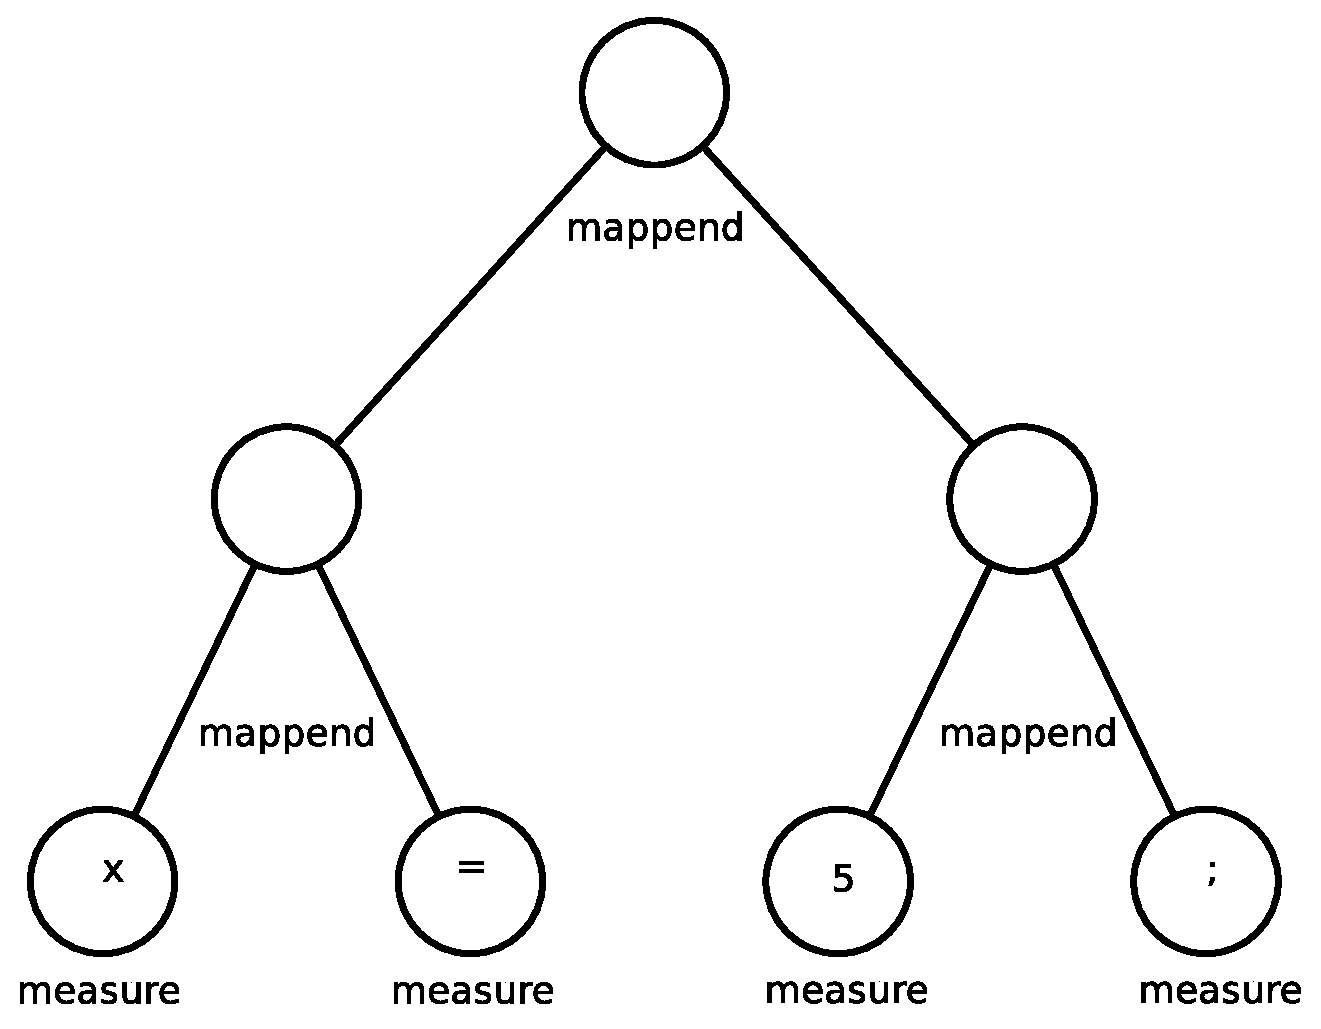
\includegraphics[width=.6\textwidth]{tree.eps}
\end{frame}

\subsection{Lexer}
\begin{frame}{Using a lexer}
    \begin{itemize}
        \item MSc thesis by Hansson and Hugo
        \item Input source code as a FingerTree
        \item Lexing by measuring \texttt{Char} $\rightarrow$
              \texttt{FingerTree} of tokens
    \end{itemize}
    % TODO: Graphic of tree with code as leaves.
\end{frame}

\subsection{Parsing}
\begin{frame}{Idea of parsing}
    \begin{itemize}
        \item Use the same approach as the lexer!
        \item Lexer measure \texttt{Char} $\rightarrow$ \texttt{FingerTree} of tokens
        \item Have the parser measure tokens $\rightarrow$ CYK entries
    \end{itemize}
\end{frame}

\begin{frame}{Pipeline of measures}
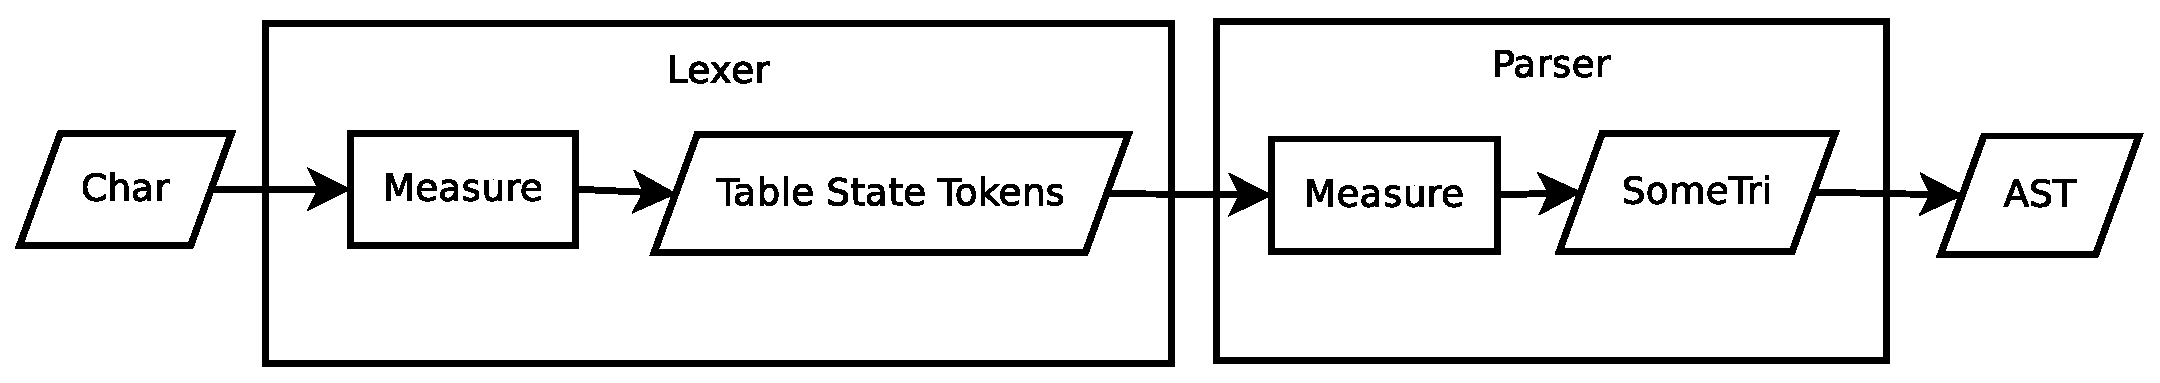
\includegraphics[width=\textwidth]{pipeline.eps}

This is done for every \texttt{Char}. Results are combined using
\texttt{mappend}.
\end{frame}

\subsection{Matrices}
\begin{frame}[fragile]{Matrix implementation}
\begin{code}
data Shape = Bin Shape Shape | Leaf
data Mat :: Shape -> Shape -> * -> * where
  Zero :: Mat x y a
  Row :: Mat x1 Leaf a -> Mat x2 Leaf a -> Mat (Bin x1 x2) Leaf a
  Col :: Mat Leaf y1 a -> Mat Leaf y2 a -> Mat Leaf (Bin y1 y2) a

data SomeTri a where
  T :: Shape' s -> Pair (Mat s s a) -> SomeTri a
\end{code}
\end{frame}

\begin{frame}{Matrix representation}
    \centering
    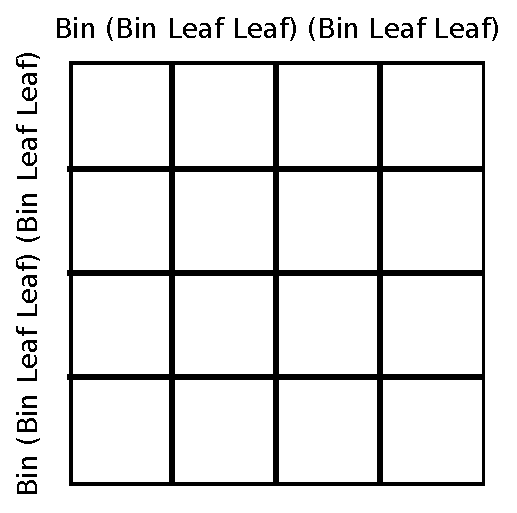
\includegraphics[width=.5\textwidth]{example-matrix-4x4.eps}
\end{frame}

\begin{frame}{Parsing as matrix multiplication}
    Existing implementation using middle element. Insufficient when such an
    element is missing. \\[.5cm]

    \begin{columns}
        \begin{column}{.4\textwidth}
            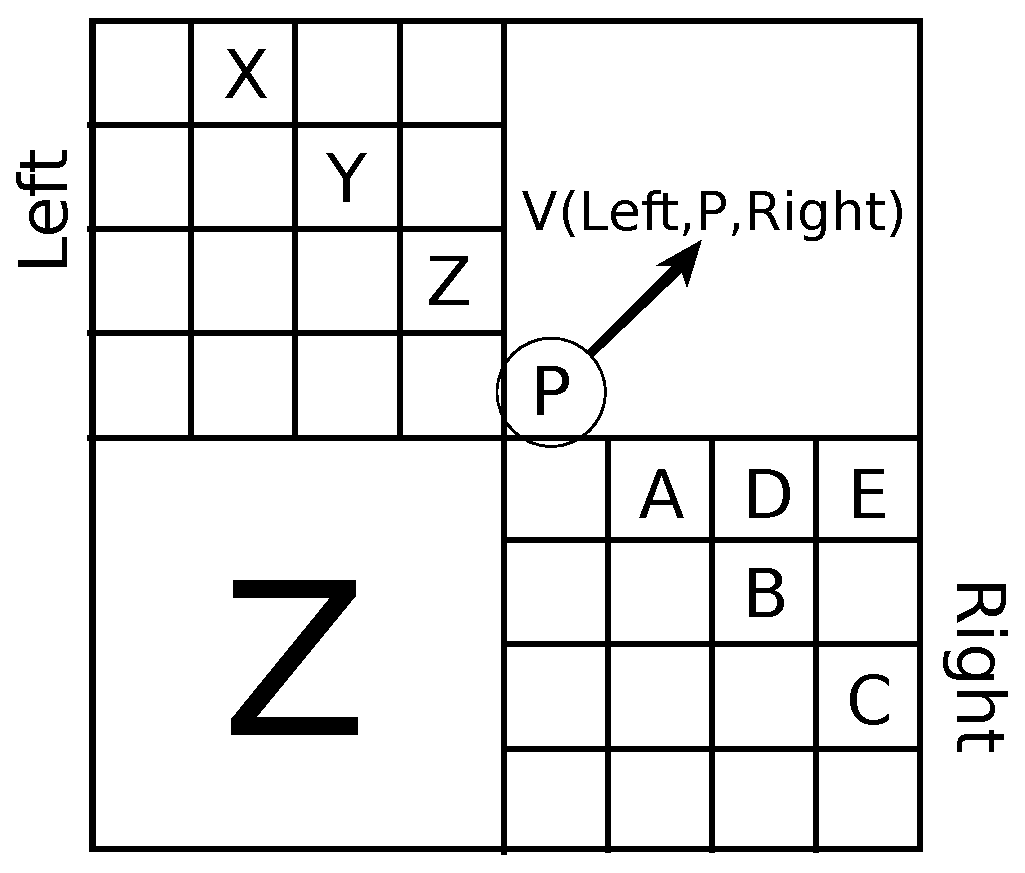
\includegraphics[width=\textwidth]{merge-with-element.eps}
        \end{column}
        \begin{column}{.4\textwidth}
            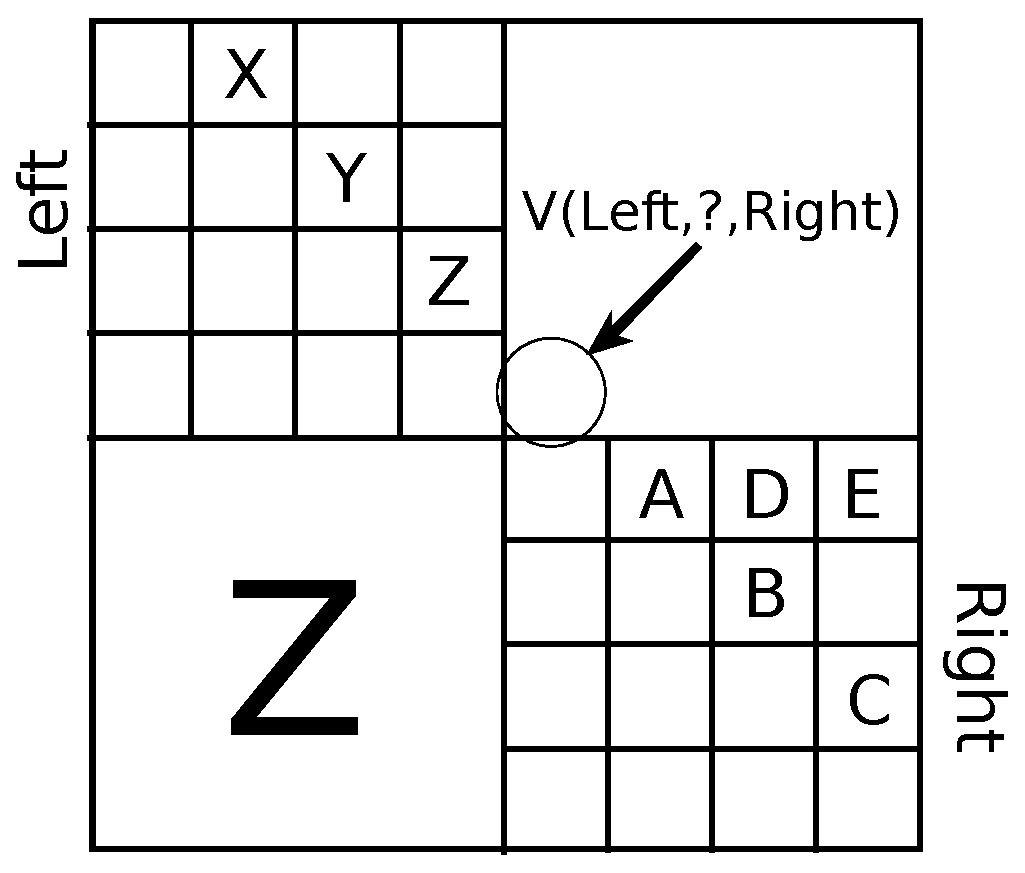
\includegraphics[width=\textwidth]{merge-without-element.eps}
        \end{column}
    \end{columns}
\end{frame}

\begin{frame}{Chopping}
    \centering
    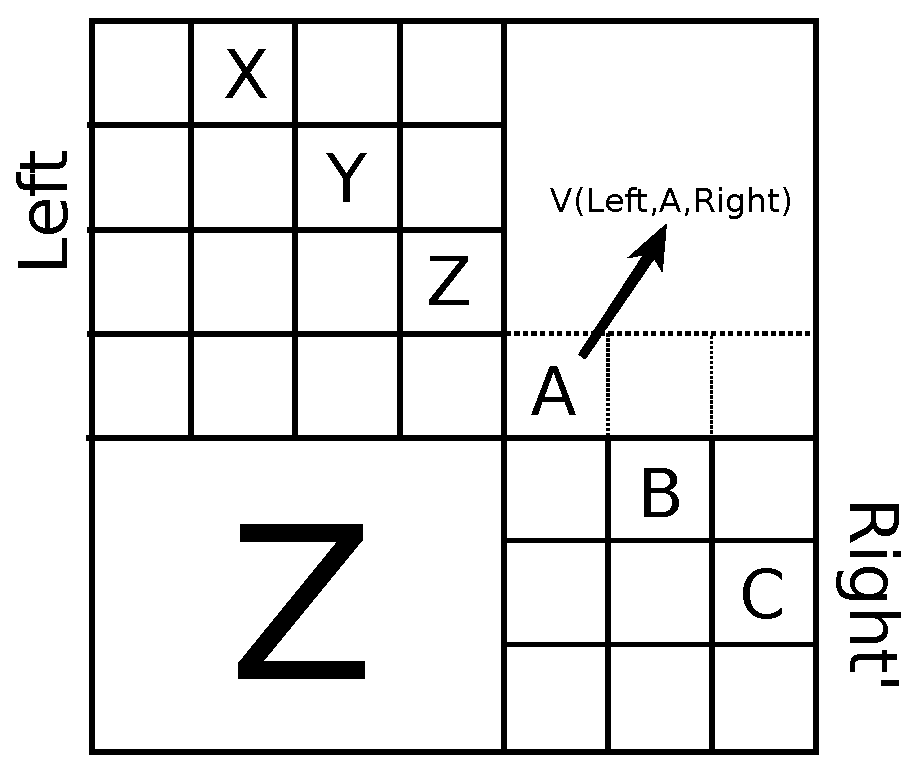
\includegraphics[width=.5\textwidth]{merge-with-chopping.eps}
\end{frame}

\begin{frame}[fragile]{Oracle}
How to select random bit?
\begin{code}
instance Monoid (SomeTri a) where
    t0 `mappend` t1 = unsafePerformIO $ do
        b <- randomIO
        return $ merge b t0 t1
\end{code}
\end{frame}

\section{Results}
\begin{frame}{Complete parser}
    \begin{itemize}
        \item Lexer and parser generated from BNFC
        \item Successfully parsing correct input
        \item Has no error handling
    \end{itemize}
\end{frame}

\subsection{Error handling}
\begin{frame}{Error handling}
    \begin{itemize}
        \item No information about the position of tokens \\ $\rightarrow$ hard to pin-point errors.
        \pause
        \item CYK may fail completely or just for some sections. \\ $\rightarrow$ has to be handled!
        \item CYK may overlap in some sections, what to do?
    \end{itemize}
\end{frame}

\begin{frame}{Overlaps}
    Overlaps may occur in the parser, depending on the input. In this example we
    can parse $j-l$ and $k-m$, but not $k-l$ and not $j-m$.

    \begin{tikzpicture}
      \pgftransformrotate{-90}
      \pgftransformscale{0.4}
      \draw (0,0) -- (10,10);
      \subt 2 6 {$A$};
      \subt 4 8 {$B$};
      \mrk 2 {$j$};
      \mrk 4 {$k$};
      \mrk 6 {$l$};
      \mrk 8 {$m$};
    \end{tikzpicture}
\end{frame}

\subsection{Measurements}
\begin{frame}{Running time}
    \begin{itemize}
        \item Hard to measure, large memory requirements!
        \item Needs to force evaluation
        \item But seems to behave
        \pause
        \item Calls for further investigation
    \end{itemize}
\end{frame}

\begin{frame}{Graph of running time}
    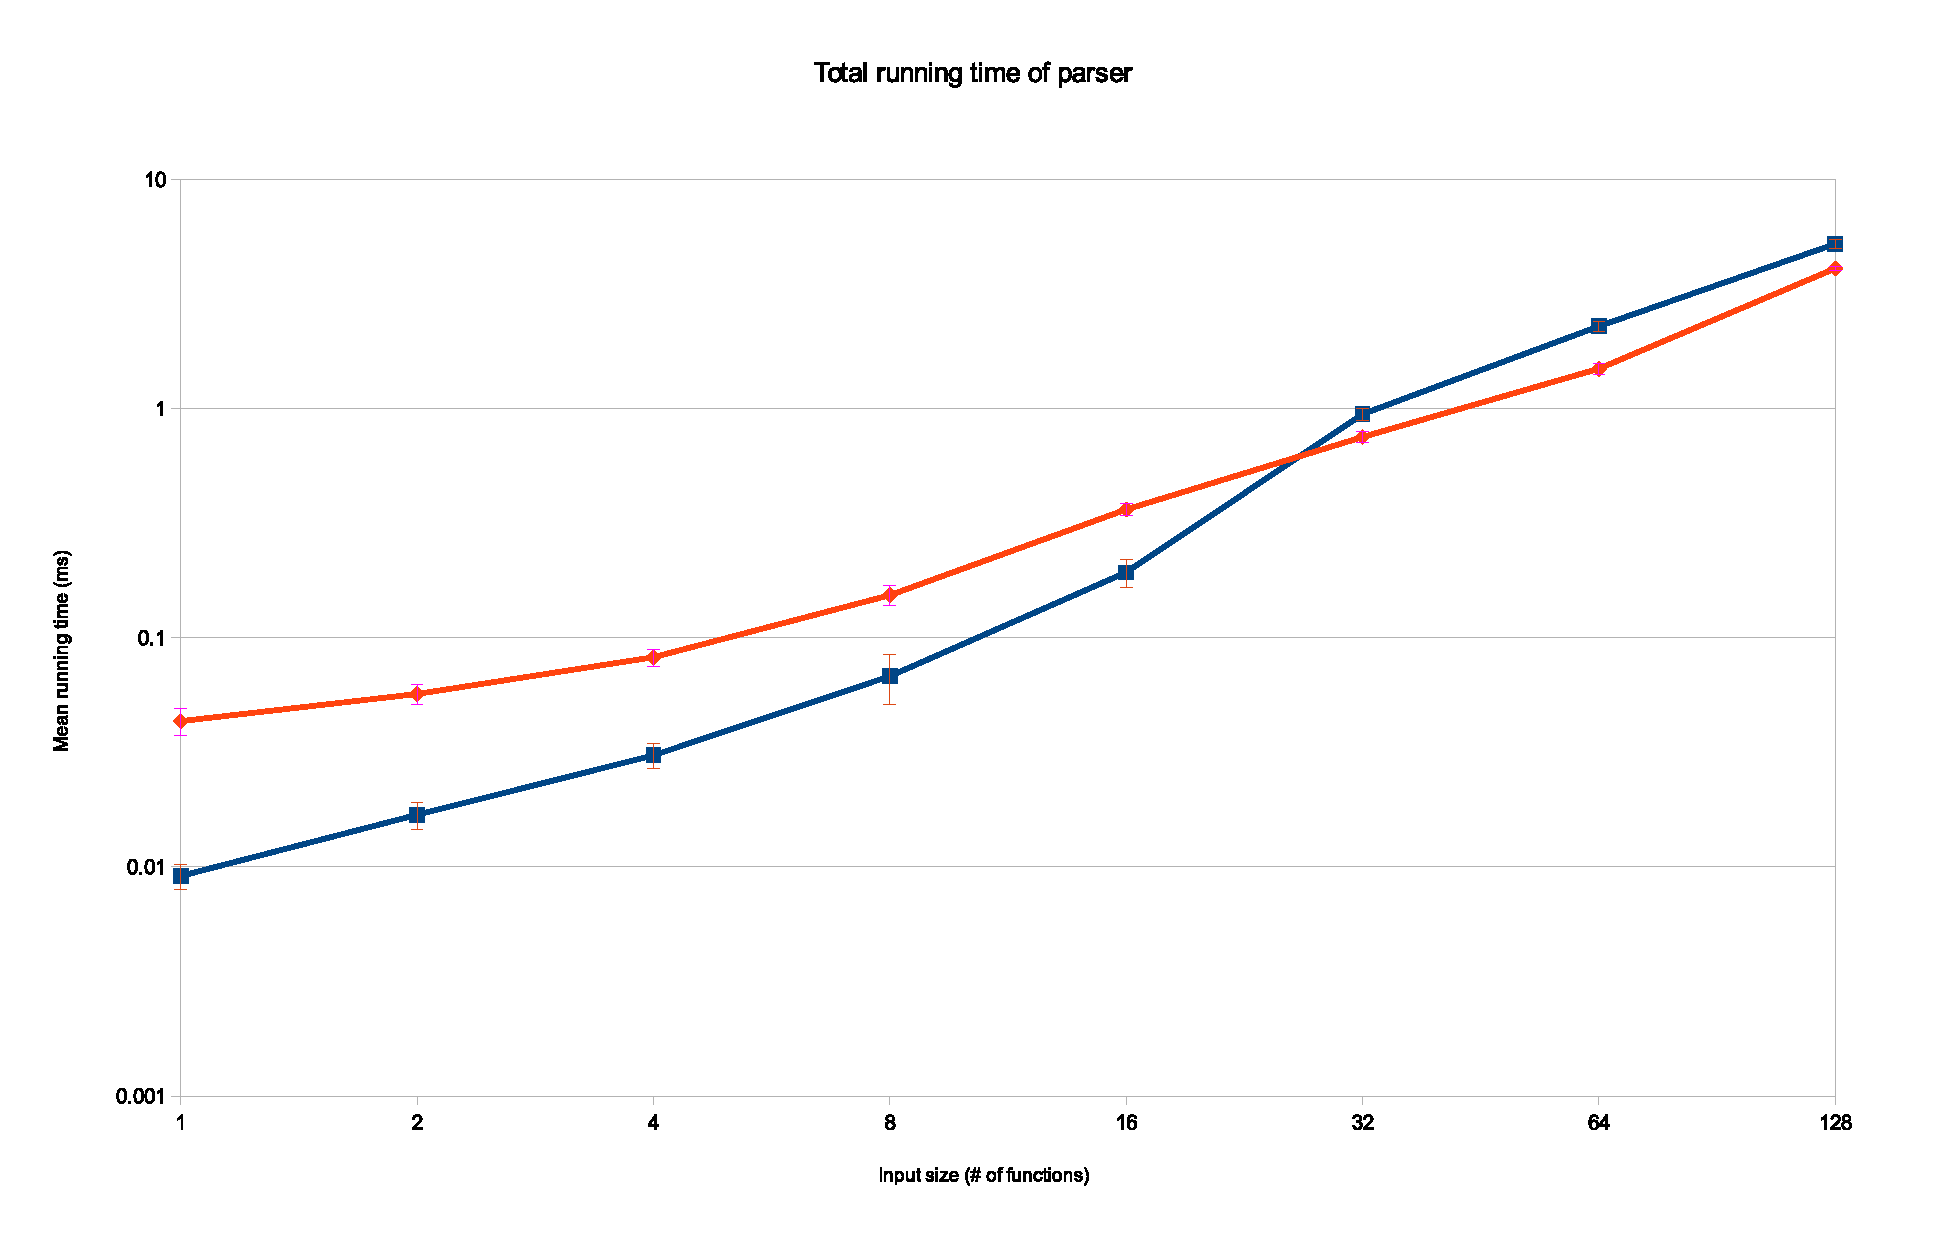
\includegraphics[width=\textwidth]{runningtime.eps}
\end{frame}

\end{document}

